\documentclass[11pt]{article}
\usepackage[margin=1in]{geometry}
\usepackage{amsmath, amssymb, bm}
\usepackage{graphicx}
\usepackage{booktabs}
\usepackage{hyperref}
\usepackage{float}
\usepackage{cite}
\usepackage{siunitx}

% Figures live in the individual report directories.
% Compile from inside report5/ with:
%   pdflatex report5.tex && pdflatex report5.tex
\graphicspath{
  {../report1/figs/}
  {../report2/figs/}
  {../report3/figs/}
  {../report4/figs/}
  {figs/}
}

\title{MIT 16.S897 --- Final Report:\\
       Attitude Determination and Control System Design\\
       for the NASA Starling 6U CubeSat}
\author{Aleksander Garbuz \and Israel Garcia}
\date{Spring 2026}

\begin{document}
\maketitle
\tableofcontents
\newpage

% ============================================================
\section{Course Project Logistics}
% ============================================================
% Pull from report1/report.tex §1

% ============================================================
\section{Mission Description and ADCS Requirements}
% ============================================================
% Pull from report1/report.tex §2

% ============================================================
\section{Spacecraft Model}
% ============================================================
% Pull from report1/report.tex §3

% ============================================================
\section{Orbital Dynamics}
% ============================================================
% Pull from report1/report.tex §4

% Example figure reference (lives in ../report1/figs/):
% \begin{figure}[H]
%   \centering
%   
\includegraphics[width=0.8\textwidth]{orbit_trajectory.png}
%   \caption{ECI orbit trajectory over 10 periods.}
% \end{figure}

% ============================================================
\section{Euler's Equation and Torque-Free Dynamics}
% ============================================================
% Pull from report1/report.tex §5

% 
\includegraphics[...]{momentum_sphere.png}
% 
\includegraphics[...]{euler_omega.png}

% ============================================================
\section{Safe-Mode Gyrostat Design}
% ============================================================
% Pull from report2/report2.tex

% ============================================================
\section{Spacecraft Dynamics with Gyrostat}
% ============================================================
% Pull from report2/report2.tex

% ============================================================
\section{Attitude Sensors}
% ============================================================
% Pull from report2/report2.tex

% 
\includegraphics[...]{sensor_noise_verification.png}
% 
\includegraphics[...]{wahba_comparison.png}

% ============================================================
\section{Static Attitude Estimation (Wahba's Problem)}
% ============================================================
% Pull from report2/report2.tex

% ============================================================
\section{Gyro Random Walk and MEKF}
% ============================================================
% Pull from report3 writeup

% 
\includegraphics[...]{gyro_random_walk.png}

% ============================================================
\section{Actuator Specifications}
% ============================================================
% Pull from report4/report4.tex §12

% ============================================================
\section{Environmental Disturbance Torques}
% ============================================================
% Pull from report4/report4.tex §13

% 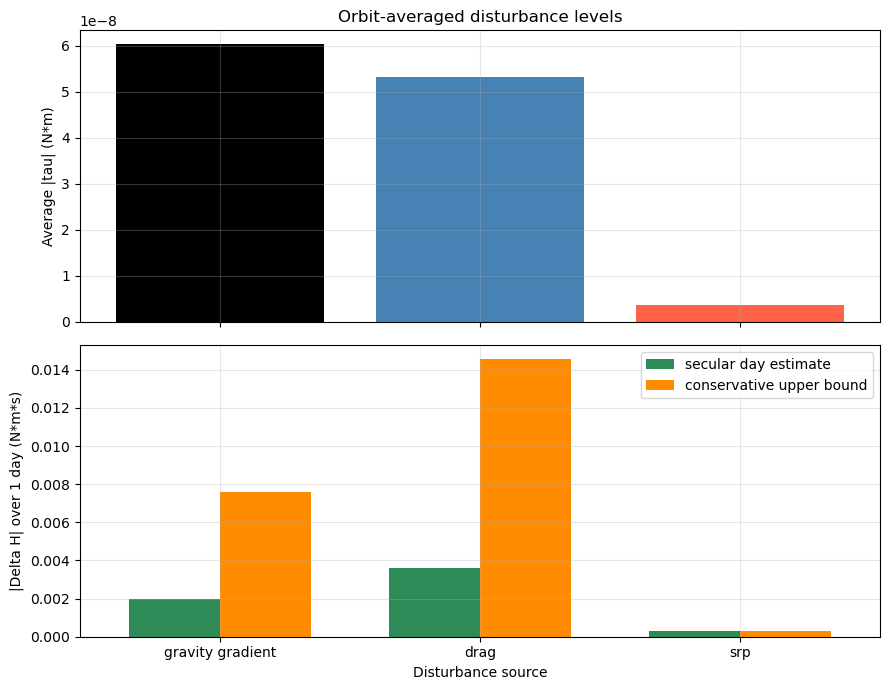
\includegraphics[...]{orbitaverageddisturbance.png}
% 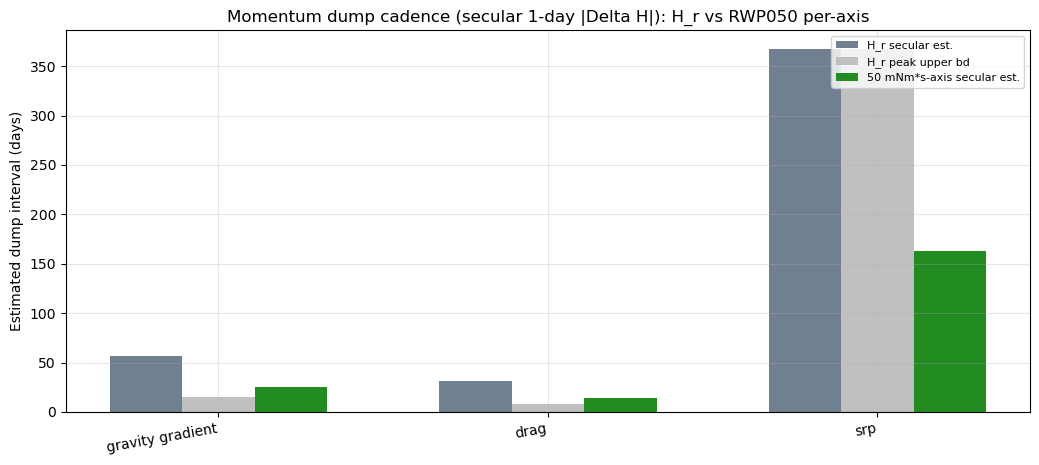
\includegraphics[...]{momuntumdumpingcadence.png}

% ============================================================
\section{Attitude Regulation}
% ============================================================
% Pull from report4/report4.tex §14

% 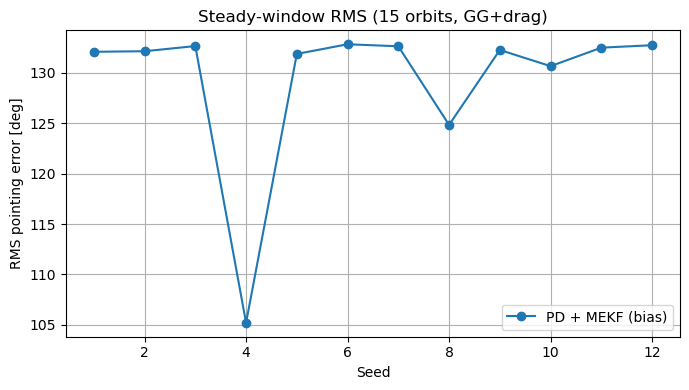
\includegraphics[...]{RMSpointingerror.png}

% ============================================================
\section{Eigen-Axis Slew}
% ============================================================
% Pull from report4/report4.tex §15

% 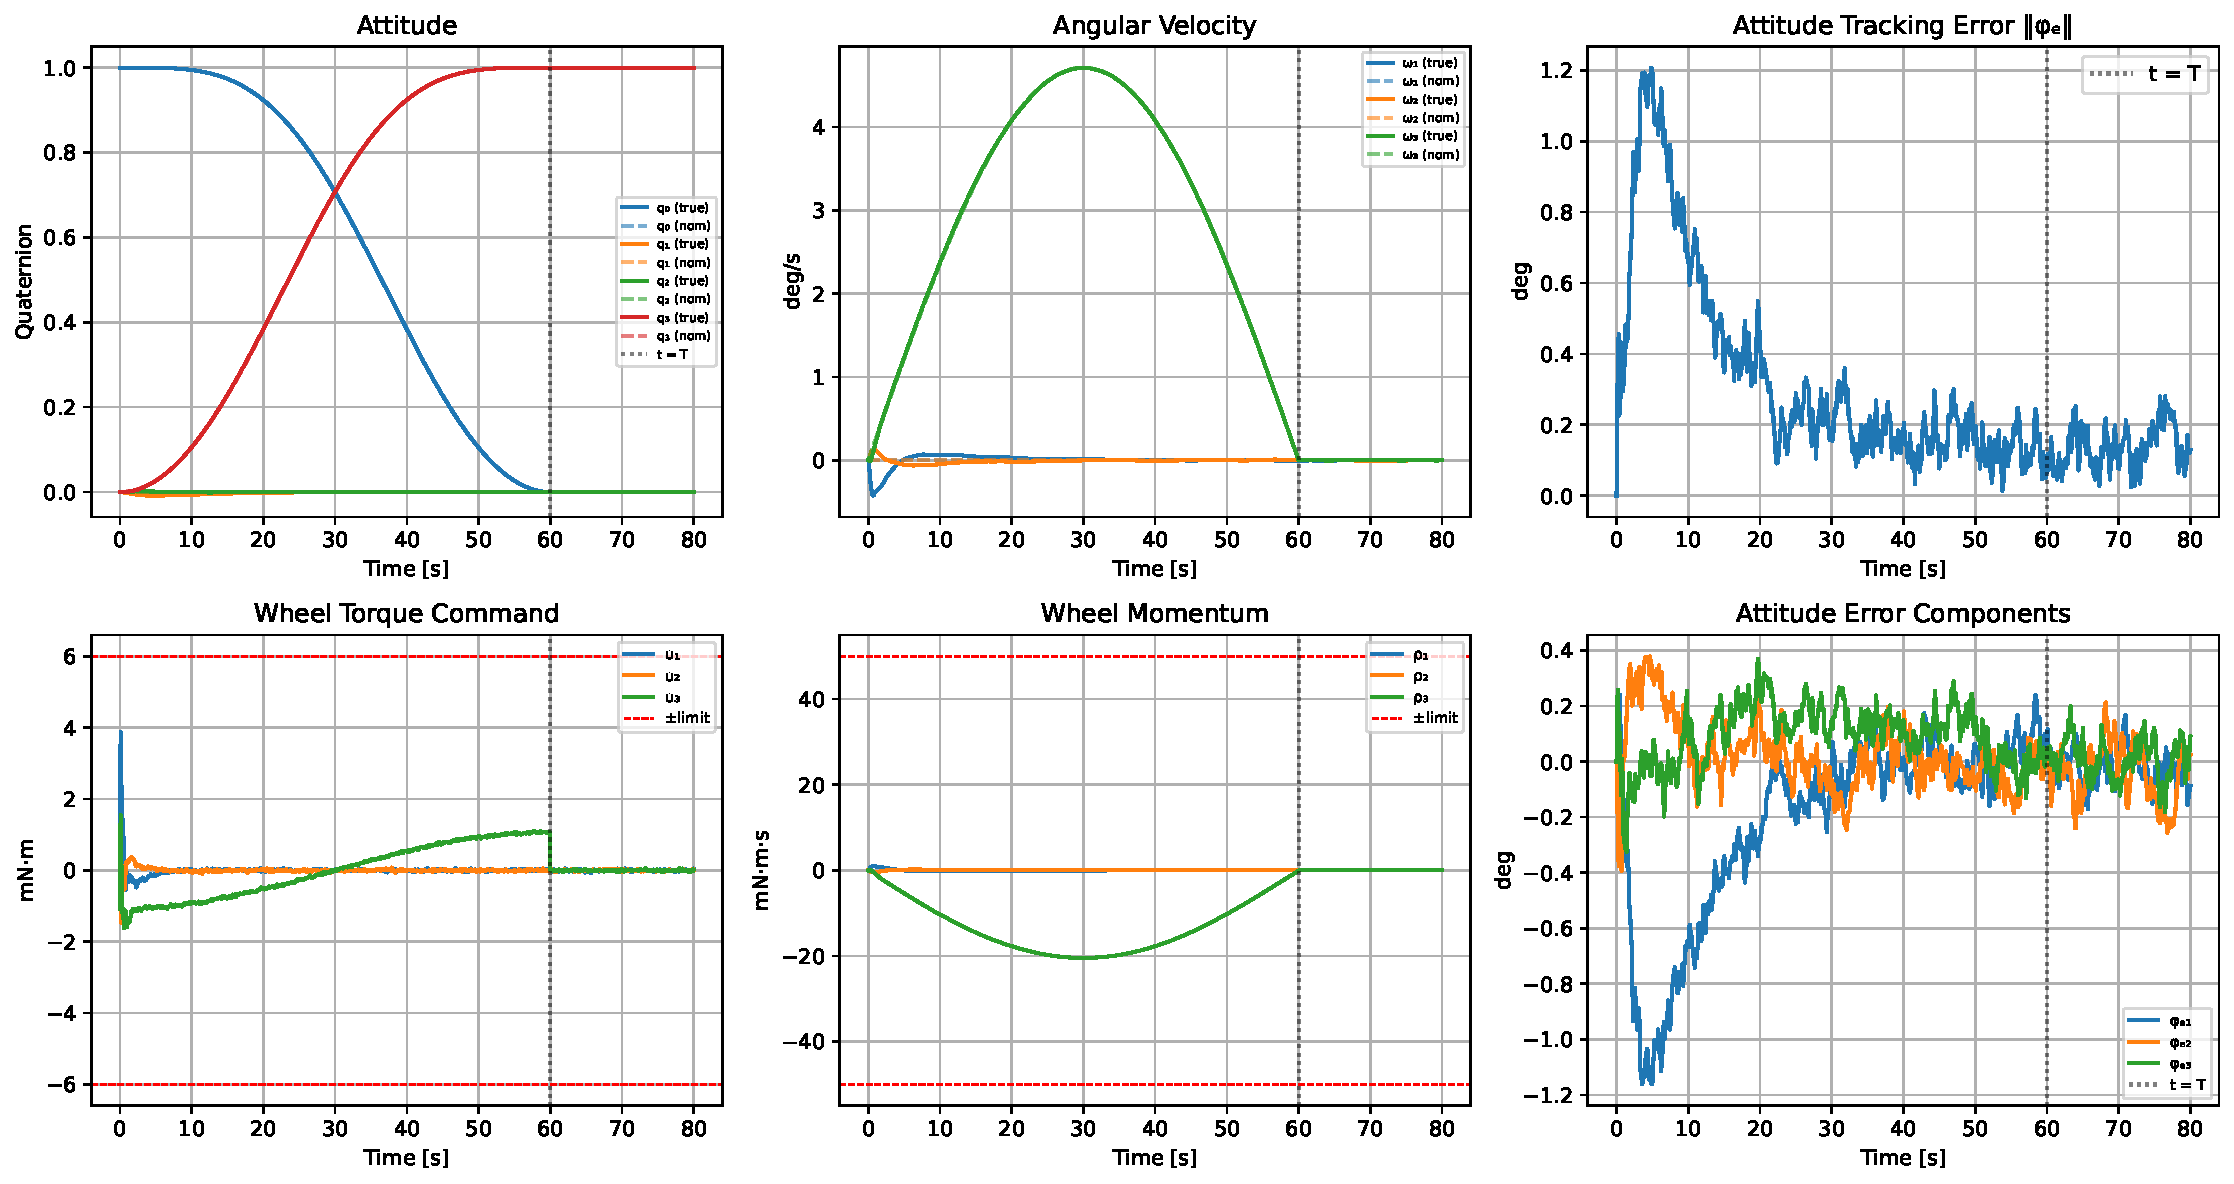
\includegraphics[...]{eigenaxis_closedloop.pdf}
% 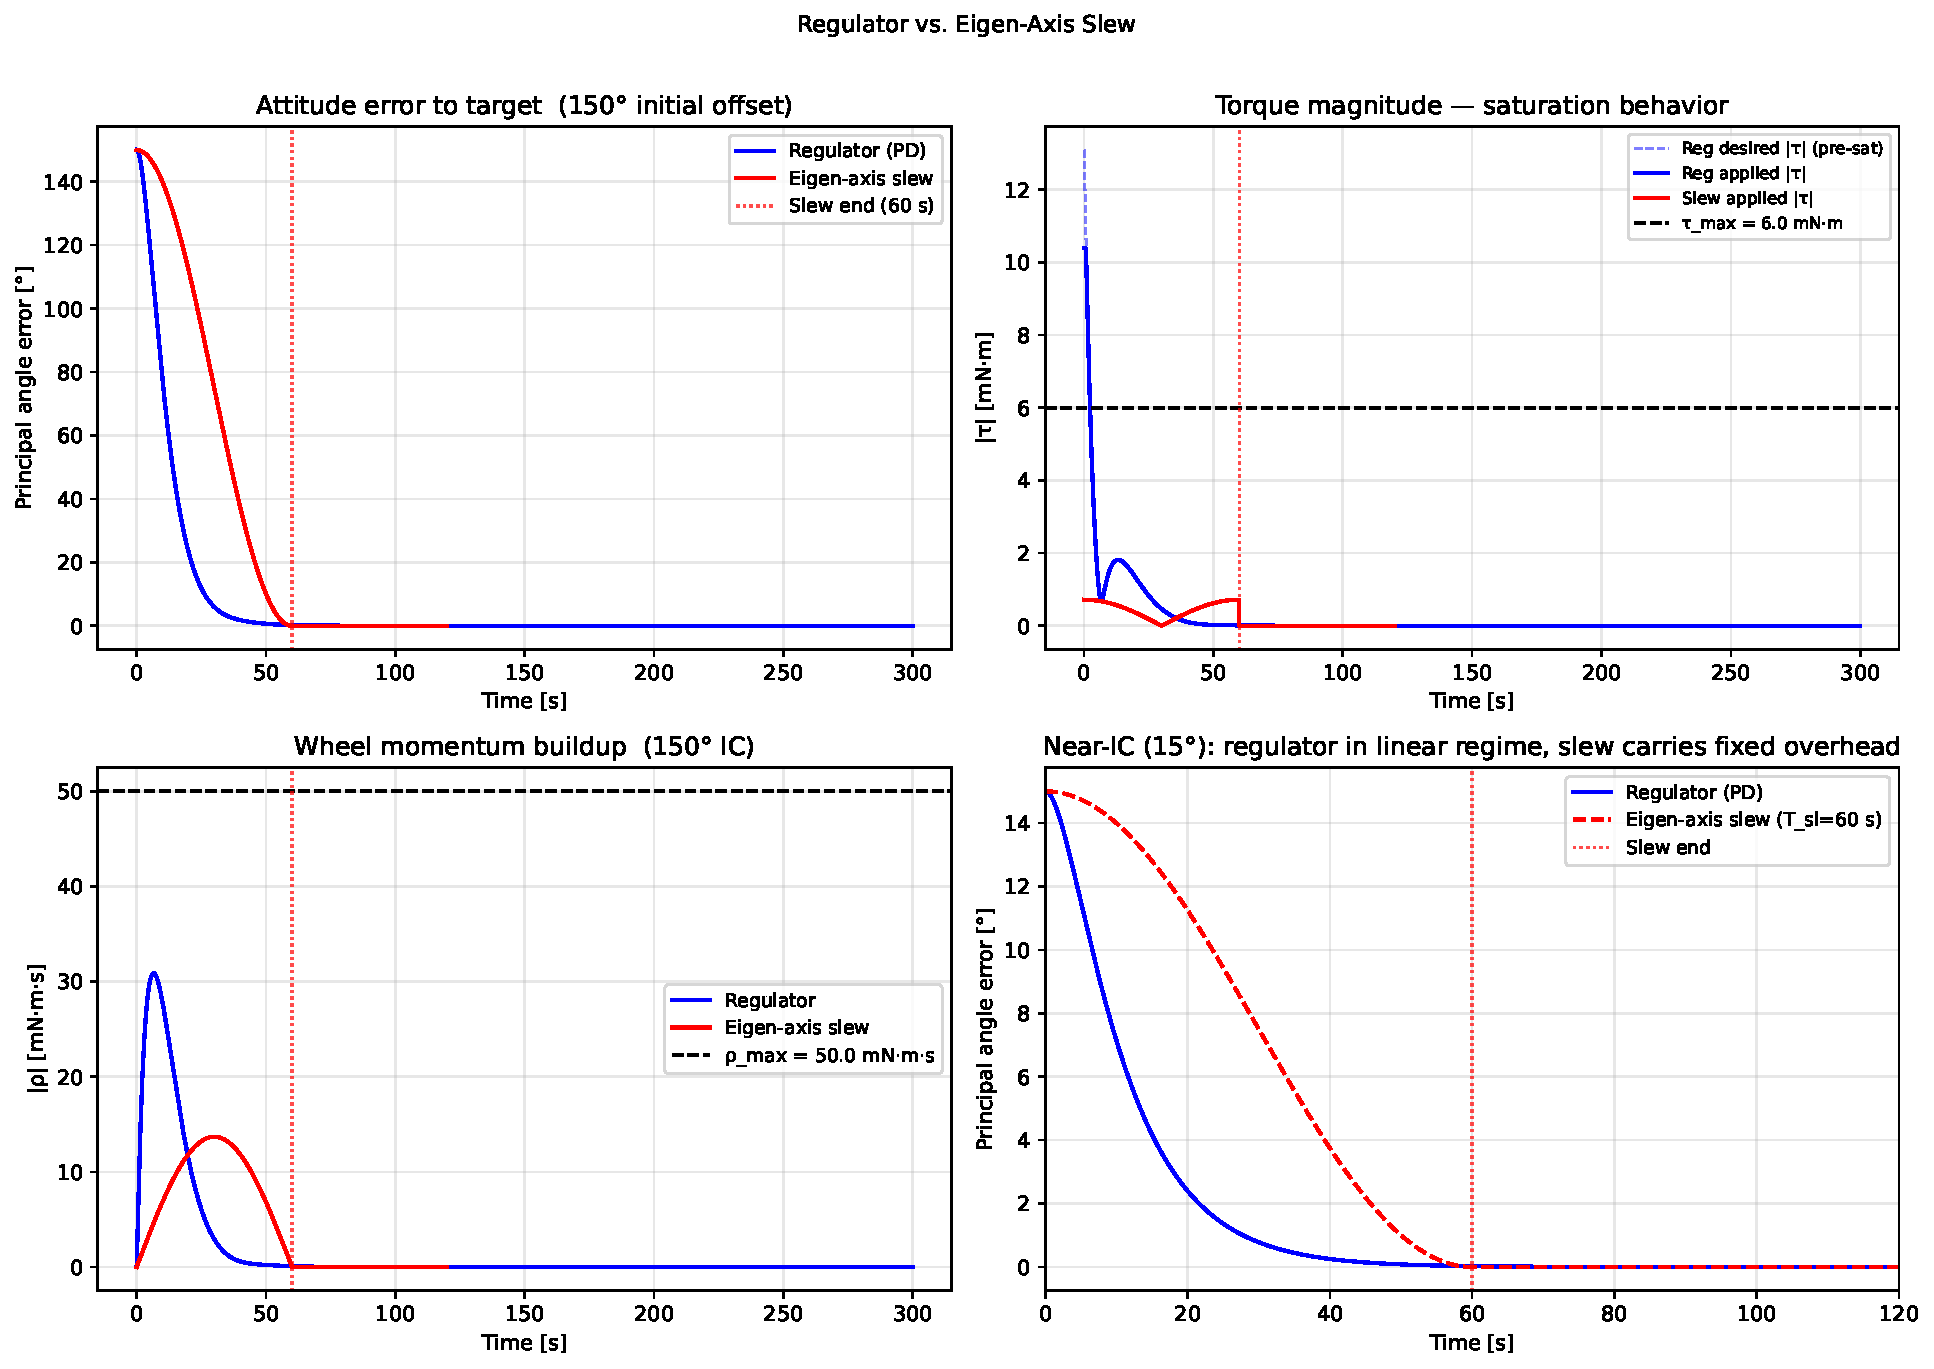
\includegraphics[...]{regulator_vs_slew_comparison.pdf}

% ============================================================
\bibliographystyle{plain}
\bibliography{refs}

\end{document}
